\begin{figure}
\centering
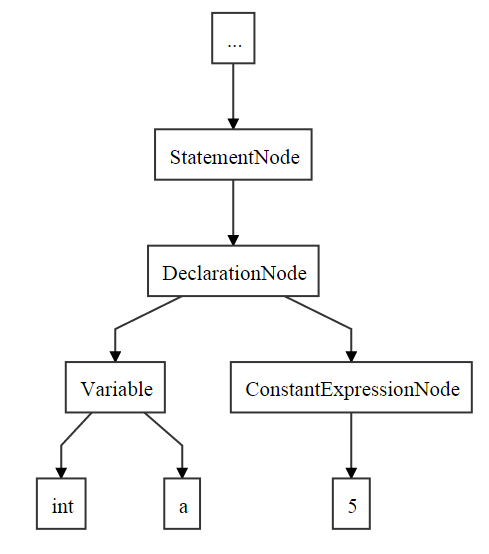
\includegraphics[width=0.5\textwidth]{figures/Trees/ASTAlone.PNG}
\caption{An \acrshort{ast} of a declaration \texttt{int a = 5;}}\label{fig:ASTAlone}
\end{figure}

\myref{fig:ASTAlone} shows a \texttt{DeclarationNode} for the expression \texttt{int a = 5;}, in the code generator this node has to be transformed into the declaration written in C. 
The syntax for this is actually the same in C as it is in \gls{gamble} but the node has been through the previous phases which means it has been statically type and scope checked, and therefore is ready to be computed.
The code from the visitor accepting a \texttt{DeclarationNode} can be seen on \myref{lst:DeclarationNodeCodeGen}.
\begin{lstlisting}[float, floatplacement=H!, caption=The visit method for visitting a DeclarationNode in the codegenerator. ,numbers=none,frame=tlrb,label={lst:DeclarationNodeCodeGen}]
@Override
public String VisitDeclarationNode(DeclarationNode node) {
    String expr = "";
    String complexType = "";
    if (node.getExpression() != null){
        resultVarStack.push(node.getVariable());
        expr = visit(node.getExpression());
        resultVarStack.pop();
    }

    if (node.getVariable().isComplex()) {
        ...
    }
    if (expr.indexOf("sclManageArgsLaunchKernel
    	(hardware, software, global_size, local_size") >= 0){
        ...
    }
    
    return complexType.length() > 0 ? complexType + expr : 
    (node.getVariable().toCcode() + " = " + expr + ";");
    }
\end{lstlisting}
Since the example \texttt{int a = 5;} is not a complex type like a matrix or vector the body of the if statement is hidden.
A check is made on the node to see if the expression which the declared variable is assigned from exists. 
Syntactically a matrix or vector can be uninitialised but this actually creates a vector or matrix filled with zeroes.
In the example the expression is not null so it goes into the body.
The result variable in which the result of the expression must be stored is pushed to a stack before visiting the expression.
In the method \texttt{VisitExpresssionNode} the top of this stack is checked to see if the result is a complex datatype or not, in the example it is not and the expression is then evaluated by visiting the nodes of the expression.
The result of the call to \texttt{VisitExpressionNode} is saved to a string \texttt{expr}.
Another if statement checks if the declaration needs a kernel and if the expression needs to be computed on the \acrshort{gpu}.
When returning the result of the call to \texttt{VisitDeclarationNode} a check is made if the complexstring has been made longer or not.
In the example \texttt{int a = 5;} is has not and therefore the string of the datatype and ID is concatenated with the assignment symbol, the substring \texttt{expr} and a semi-colon, before finally being returned.



